% =====================================================================
%  NPM3D project report -- revised version
%  Author: Nassim Arifette
%  Build:  pdflatex rapport_npm3d.tex  (twice, for references)
%
%  All numbers in Section 6 come from
%      python -m spatial_reasoning.run_experiments --source synthetic
%  aggregated over seeds 0,1,2 in spatial_reasoning/results/summary.md
% =====================================================================

\documentclass[11pt,a4paper]{article}

\usepackage[utf8]{inputenc}
\usepackage[T1]{fontenc}
\usepackage[english]{babel}
\usepackage{lmodern}
\usepackage{microtype}
\usepackage{amsmath,amssymb}
\usepackage{booktabs}
\usepackage{xcolor}
\usepackage{enumitem}
\usepackage{tikz}
\usetikzlibrary{arrows.meta,positioning}
\usepackage[margin=2.5cm]{geometry}
\usepackage[hidelinks]{hyperref}

\newcommand{\code}[1]{\texttt{\small #1}}

\title{\textbf{Low-cost LiDAR spatial reasoning:\\
learned answers versus explicit geometric operations}}
\author{Nassim Arifette\\
\small MVA --- Nuages de Points et Modélisation 3D (NPM3D)}
\date{\today}

\begin{document}
\maketitle

\begin{center}
\fbox{\begin{minipage}{0.92\textwidth}
\small\textbf{Status of the numbers in this version.} Section~6 reports the
\emph{synthetic} campaign, under $45^{\circ}$ octant sectors
(\code{spatial\_reasoning/results/all\_results.json}). Work since has moved to
real nuScenes-QA questions under that benchmark's six $60^{\circ}$ sectors, a
convention since checked against the gold answers rather than assumed. Under
those conditions the measured figures differ from the ones below --- the
learned baselines do not reliably beat a scene-blind prior, and swapping
ground-truth objects for detections barely moves them. The current state is
tracked in \code{spatial\_reasoning/results/state\_of\_results.md}, and the
comparison this report argues for --- one language model answering directly
against the same model writing an executable program --- is Section~7, on real
nuScenes-QA questions. The synthetic results in Section~6 are kept because the
argument they illustrate is unchanged; they should not be cited as results on
nuScenes-QA.
\end{minipage}}
\end{center}

\vspace{1em}

\begin{abstract}
\noindent
LiDAR-LLM \cite{lidarllm} couples a frozen LiDAR encoder to a large language
model so that spatial questions about a driving scene can be answered in
natural language. Our original project reimplemented a reduced version of that
architecture and showed, honestly, that it could not be trained on the
hardware available: a GPT-2 answer head on filtered nuScenes-mini data, with no
completed training run. This revised report changes the question rather than
the hardware. Holding perception fixed --- consuming 3D detections computed
once and never retrained --- we ask whether a spatial question is better
answered by \emph{learning} the answer or by \emph{computing} it: parse the
question into an explicit program, select the relevant objects, and apply a
geometric operation. Four systems are compared under one protocol with
scene-level splits: a question-only language prior, a deep-sets answer
classifier, a differentiable counter, and a parameter-free symbolic program.
On a balanced synthetic corpus the symbolic system reaches $0.916$ accuracy
against $0.656$ for the best learned system --- which does not beat the
question-only prior --- with a counting error of $0.13$ against $0.53$, no
trained parameters, and three times less inference time. Contrast pairs make
the gap starker still: $0.643$ against $0.08$ and below. Every symbolic error
traces to perception, none to question understanding or geometry. The whole
study runs on a CPU in under a minute per configuration, which is the point:
the contribution is a comparison that is affordable, reproducible, and capable
of a negative result.
\end{abstract}

% =====================================================================
\section{Introduction}
% =====================================================================

Interpreting a LiDAR scene in natural language is attractive for autonomous
driving: a system that can answer ``how many cars are ahead of us?'' exposes
its scene understanding in a form a human can audit. LiDAR-LLM
\cite{lidarllm} pursues this by aligning a LiDAR representation with the
embedding space of a language model through a three-stage curriculum ---
cross-modal alignment, perception learning, and high-level instruction tuning
--- with GPT-4 \cite{gpt4} used to improve the captions that form the training
data, and LLaMA-7B as the model that learns from LiDAR.

Our first report reimplemented a reduced version of this architecture. Section
\ref{sec:original} restates what that implementation did and, more usefully,
what it failed to establish. Section \ref{sec:question} then argues for a
different question, one the same hardware can actually answer.

The shift is motivated by an observation about counting and directional
questions. When the correct answer to ``how many cars are in front?'' is
determined by the detected object list and a geometric predicate, asking a
generative model to emit the digit is asking it to re-derive, inside its
weights, a computation that is already exact and essentially free. Whether
that re-derivation buys anything is testable, and this report tests it.

% =====================================================================
\section{The original re-implementation and what it did not show}
\label{sec:original}
% =====================================================================

The first version of this project implemented the LiDAR-LLM pipeline in
reduced form: a small PointNet as the LiDAR encoder, a view-aware transformer
with six view-position embeddings, an MLP adapter projecting into the token
embedding space, and GPT-2 \cite{gpt2} fine-tuned with LoRA \cite{lora} as the
language model. Data came from nuScenes-mini \cite{nuscenes} filtered to the
samples present in the mini split, together with nuScenes-QA \cite{nuscenesqa}
questions: 323 training samples from 8 scenes and 81 validation samples from 2
scenes.

The honest summary is that it produced a debugged pipeline and no evidence.
Training ran on laptops with roughly 6\,GB of RAM and no GPU. The functional
check was that the model could be driven to emit a fixed string regardless of
the LiDAR input, which shows that gradients flow and nothing more. A
distillation stage was implemented and its loss decreased, which again shows
that the optimisation is wired correctly, not that the student retains any
spatial ability.

Three weaknesses matter for what follows.

\paragraph{The evaluation could not separate competence from priors.}
nuScenes-QA answers are heavily skewed towards ``no'' and small integers. With
no question-only control, an accuracy figure cannot distinguish a model that
reads the scene from one that has learned the answer distribution. Real-3DQA
\cite{real3dqa} demonstrates how severe this is: on SQA3D a model fine-tuned on
question-answer pairs \emph{with no 3D input at all} matches or beats existing
3D-LLMs, and once the blind-answerable questions are filtered out, LEO's exact
match collapses from $49.4\%$ to $14.3\%$ and Chat-Scene's to $17.0\%$.

\paragraph{The split invited leakage.}
Splitting questions rather than scenes places different questions about the
same LiDAR sample on both sides of the split, so memorising ``this scene has
three cars'' is rewarded.

\paragraph{The target task did not need a language model.}
Counting, existence and directional questions have answers that are functions
of the object list. Nothing about them requires text generation.

% =====================================================================
\section{A question the available hardware can answer}
\label{sec:question}
% =====================================================================

We fix perception and vary only the reasoning stage. Detections are computed
once --- CenterPoint-style 3D boxes \cite{centerpoint}, as shipped with
nuScenes-QA, or ground-truth boxes for an oracle condition --- and every system
receives exactly the same object list. The research question is:

\begin{quote}
\emph{At fixed perception and comparable budget, is it better to learn the
answer to a spatial question directly, or to select objects and then apply
explicit geometric operations?}
\end{quote}

This is narrower than ``can LiDAR-LLM be made smaller?'', and that is
deliberate: it yields an interpretable result either way. If explicit
computation wins, the learned head was spending capacity on arithmetic. If the
learned head wins, robustness to imperfect detections outweighs exactness ---
the more interesting finding, which the perturbation study of Section
\ref{sec:probes} is designed to detect.

\paragraph{Relation to existing work.}
Separating language understanding from geometric execution is not new, and our
contribution is not the idea but its controlled measurement. ZSVG3D
\cite{zsvg3d} already produced programs from language for zero-shot 3D
grounding, composing view-independent, view-dependent and functional modules.
KLDrive \cite{kldrive} is the closest system to the design tested here: it
merges multi-source evidence into a scene knowledge graph and lets a frozen
Qwen3-7B agent reason over it through a Plan--Execute--Observe loop restricted
to a fixed action space, reaching $65.04\%$ overall accuracy on nuScenes-QA and
$64.46\%$ on counting against $18.45\%$ for its strongest baseline.
Retrieve-to-Localize \cite{retrieve2localize} makes the complementary argument
for coordinates: rather than generating them as text, it retrieves
language-conditioned spatial proposals and refines the position from local
LiDAR points. BEV-LLM \cite{bevllm} extends LiDAR-LLM directly --- the authors
state that their method builds upon it --- by adding camera images through
BEVFusion and an absolute positional encoding, with a frozen Llama and a LoRA
adapter. NuScenes-SpatialQA \cite{nuscenesspatialqa} builds spatial questions
from nuScenes scene graphs and finds that a spatially enhanced VLM improves on
qualitative questions while remaining uncompetitive on quantitative ones, which
is precisely the counting gap this report targets. 3DGraphLLM
\cite{3dgraphllm} learns a scene-graph representation carrying semantic
relations between objects, evaluated indoors on ScanRefer, Multi3DRefer,
ScanQA, SQA3D and Scan2Cap.

Two things prevent a direct numerical comparison with our results. First,
these systems change more than the reasoning module: KLDrive's accuracy is
obtained with three detectors (RayDN, FocalFormer3D and IS-Fusion) over 39{,}704
selected questions under a random $8{:}2$ split that is not stratified by
scene, so part of the gain is perception and part is protocol. Second, ``frozen
LLM'' does not mean cheap: KLDrive runs on RTX A6000 GPUs,
Retrieve-to-Localize trains on four A6000s with 48\,GB each, and BEV-LLM's
1B-parameter variant takes 48 hours on eight A100s despite freezing both
BEVFusion and the language model. The experiment reported below runs in 49
seconds on a CPU. It is a much smaller claim, measured properly, rather than a
larger claim taken on faith.

% =====================================================================
\section{Method}
% =====================================================================

\subsection{Object-level scene representation}

A scene is a list of objects, each with a canonical class (the ten nuScenes
detection classes), a centre, a box size, a yaw and a detection score. All
coordinates are in the ego frame: $x$ forward, $y$ left, $z$ up. Detection
results released for nuScenes are in global coordinates, so the conversion
through the sample's ego pose is performed explicitly and in one place; a
mistake there mirrors the scene and would be indistinguishable from a reasoning
failure.

\subsection{Directions as bearing sectors}

Directional words are $45^{\circ}$ bearing sectors centred on front,
front-left, left, back-left, back, back-right, right and front-right. Sectors,
rather than axis-aligned half-planes, give two properties we rely on: an object
belongs to at most one named direction, and a car $40$\,m ahead and $2$\,m to
the left is ``front'' rather than simultaneously ``front'' and ``left''.
Objects closer than $1$\,m to the ego origin are excluded from directional
queries, because a $10$\,cm localisation error flips the sign of their bearing.

Relative directions (``left of the truck'') are ambiguous between the viewer's
frame and the object's own frame. Both are implemented and the choice is an
explicit parameter; the viewer-centric reading is the default, matching
nuScenes-QA.

\subsection{From question to program}

A rule-based parser maps a question onto a structured query: an operation
(\textsc{count}, \textsc{exists}, \textsc{compare}), a category or category
group, and a region (anywhere, a direction sector, near, far, or a radius). The
parser never sees the scene, which is what makes the error decomposition of
Section \ref{sec:errors} possible: a wrong answer is a comprehension error if
and only if the parser produced the wrong query, independently of what the
detector saw.

The parser \emph{declines} questions outside its grammar instead of guessing.
Coverage and accuracy are therefore separate numbers, and the results contain
two symbolic variants: one that abstains, and one that falls back to the
majority training answer so that it is directly comparable to a model which
always emits something.

\subsection{Execution}

Executing a query is a filter followed by an arithmetic operation. It is
deterministic, has no learned parameters, and returns the list of objects it
selected, which is what allows an error to be attributed to perception rather
than to reasoning. A definite reference whose resolution is ambiguous (``the
truck'', when the scene contains three) is refused rather than resolved by
taking the first match: silently choosing would hide the failure and inflate
the score.

\begin{figure}[t]
\centering
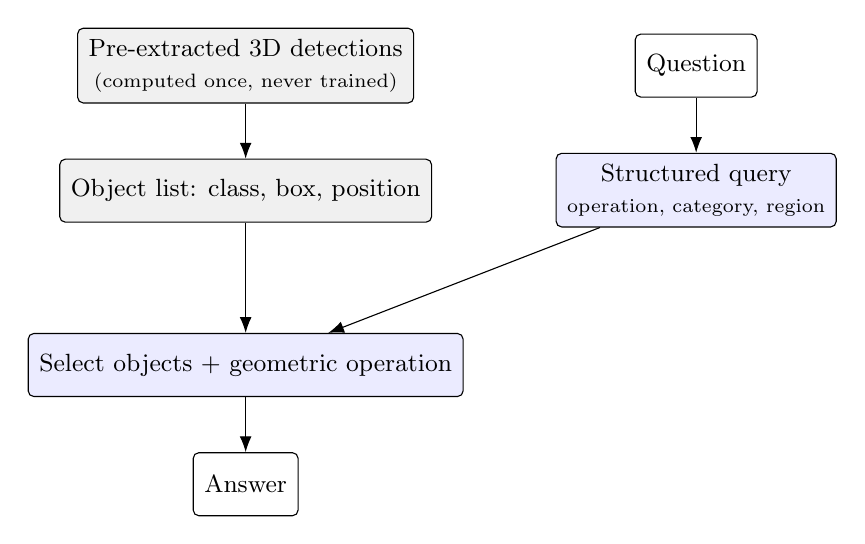
\begin{tikzpicture}[
  node distance=7mm,
  box/.style={draw, rounded corners=2pt, align=center, inner sep=4pt,
              minimum height=8mm, font=\small},
  fixed/.style={box, fill=gray!12},
  learn/.style={box, fill=blue!8},
  arr/.style={-{Latex[length=2mm]}}
]
\node[fixed] (det)  {Pre-extracted 3D detections\\\scriptsize(computed once, never trained)};
\node[fixed, below=of det] (objs) {Object list: class, box, position};
\node[box, right=28mm of det] (q) {Question};
\node[learn, below=of q] (parse) {Structured query\\\scriptsize operation, category, region};
\node[learn, below=14mm of objs] (exec) {Select objects $+$ geometric operation};
\node[box, below=of exec] (ans) {Answer};

\draw[arr] (det)   -- (objs);
\draw[arr] (q)     -- (parse);
\draw[arr] (objs)  -- (exec);
\draw[arr] (parse) -- (exec);
\draw[arr] (exec)  -- (ans);
\end{tikzpicture}
\caption{The symbolic pipeline. Grey is fixed perception, shared with every
baseline; blue is the only part that varies between the compared systems. No
language model appears anywhere.}
\label{fig:pipeline}
\end{figure}

\subsection{The learned baselines}

Three learned systems consume the same object lists.

\begin{description}[leftmargin=1.4em,style=nextline]
\item[Question-only.] A bag-of-words encoding of the question feeds an MLP
  over the answer vocabulary. It never sees the scene. Its accuracy is the
  language prior, and it is the threshold any other system must clearly clear
  before it can be said to use the 3D input.
\item[Deep sets.] The question vector is concatenated to every object feature;
  a shared encoder is applied per object; sum and mean pooling are concatenated
  and classified. Sum pooling carries cardinality, which counting needs; mean
  pooling is scale-stable. This is the ``predict the answer directly''
  condition --- a miniature of the LiDAR-LLM answer head without the language
  model.
\item[Deep sets $+$ explicit counter.] The same backbone with an additional
  per-object relevance head in $[0,1]$ whose sum is trained, with an $L_1$
  loss, to equal the count. The inductive bias is ``an answer of $N$ comes from
  $N$ objects'', without hard-coding which ones.
\end{description}

The text encoder is deliberately the cheapest possible: CRC32-hashed unigrams
and bigrams, no pretrained weights. The experiment is about where the
computation happens, and a gain that required a large text encoder would
confound that.

% =====================================================================
\section{Experimental protocol}
% =====================================================================

\subsection{Data}

\textbf{Synthetic (used here).} Scenes are sampled with nuScenes-like class
frequencies and sizes, and questions are generated \emph{from} queries, so the
gold program of every question is known --- which is what makes the
comprehension/geometry split possible. A detector-failure model (12\% drops,
5\% duplicates, $0.6$\,m localisation jitter) turns the ground-truth list into
the ``detected'' list the systems consume, so an oracle and a realistic
perception condition exist for every sample. Ten scenes, 20 samples each, 8
questions per sample: 1600 questions over 200 samples.

A second, \emph{degenerate} setting is reported alongside. Without balancing,
75\% of answers mean ``nothing is there'' --- a question about a rare class
inside a $45^{\circ}$ sector is almost always answered ``none''. The default
setting caps that share at 35\%. The comparison between the two settings is
itself a result, and it reproduces Real-3DQA's finding on our own data.

\textbf{nuScenes.} The same code runs on released CenterPoint detections plus
a nuScenes-QA style question file, with ground-truth boxes optionally supplied
for the oracle condition. Those runs are not reported here.

\subsection{Splits, metrics, probes}

Splits are by scene, never by question. Accuracy is exact match, with an
abstention counted as an error; for counting questions we also report mean
absolute error, which separates ``4 instead of 3'' from ``11 instead of 3''.
Cost is wall-clock time per item, measured identically for all systems; the
one-off cost of running the detector is excluded from all systems equally.
Three probes are run.

\label{sec:probes}
\paragraph{Contrast pairs.} The same question text paired with two samples
having different correct answers; a pair counts only if both are right. A
system answering from the language prior cannot score here.

\paragraph{Counterfactual moves.} One object is moved from one sector to
another and the reference answer is recomputed. We report accuracy and how
often the answer changed at all, because failing to react is the more
diagnostic failure. The reference answers come from the same executor the
symbolic system uses, so that system scores $1.000$ by construction; the probe
is evidence about the learned baselines and a regression test for the symbolic
one.

\paragraph{Perception degradation.} Detections are dropped, duplicated and
jittered, one failure mode at a time. This perturbs detections, not the point
cloud, and therefore models detector failures rather than sensor noise.

\subsection{Error decomposition}
\label{sec:errors}

Each symbolic error is attributed to a stage: \textbf{perception} (the same
parsed program on ground-truth objects gives the right answer),
\textbf{comprehension} (the parsed query differs from the gold query),
\textbf{geometry} (query and objects both right, region maths wrong),
\textbf{declined} (outside the grammar), or \textbf{unattributed} (no oracle
boxes or gold program available).

% =====================================================================
\section{Results}
% =====================================================================

All figures are means over seeds $0,1,2$ with population standard deviations,
test split $n=320$ per seed. The balanced setting has $37.1\%$ trivial answers
and a majority-answer accuracy of $0.296$; the degenerate setting has $75.0\%$
and $0.412$. Parser coverage is $1.000$ in both, by construction: the questions
were generated from the same grammar, so coverage here measures the instrument,
not the language.

\begin{table}[h]
\centering
\caption{Main comparison at fixed perception, balanced setting. All systems see
the same detections and the same scene-level split.}
\label{tab:main}
\small
\begin{tabular}{lrrrr}
\toprule
System & Accuracy & Count MAE & Params & ms/item \\
\midrule
Majority answer          & 0.296 & --- & 0 & --- \\
Question only            & $0.656 \pm 0.012$ & $0.722 \pm 0.093$ & 35\,863 & 0.68 \\
Deep sets                & $0.655 \pm 0.020$ & $0.654 \pm 0.088$ & 120\,855 & 0.88 \\
Deep sets $+$ counter    & $0.644 \pm 0.018$ & $0.534 \pm 0.035$ & 129\,176 & 1.09 \\
\textbf{Symbolic}        & $\mathbf{0.916 \pm 0.027}$ & $\mathbf{0.132 \pm 0.053}$ & \textbf{0} & \textbf{0.23} \\
\bottomrule
\end{tabular}
\end{table}

Three things stand out in Table \ref{tab:main}. The symbolic system is $26$
accuracy points above the best learned system and its counting error is four
times smaller, with no trained parameters and three times less inference time.
Neither learned model beats the question-only control: deep sets matches it to
within noise and the counter is marginally below it. And the counter does what
it was designed to do, but only partially --- it cuts the counting error from
$0.654$ to $0.534$ without improving accuracy, so the inductive bias improves
the magnitude of the estimate without making it exact.

\begin{table}[h]
\centering
\caption{Consistency probes, balanced setting. Pair accuracy requires both
members of a contrast pair to be correct. The symbolic system's counterfactual
score is $1.000$ by construction (Section \ref{sec:probes}).}
\label{tab:probes}
\small
\begin{tabular}{lrrr}
\toprule
System & Pair accuracy & Counterfactual acc. & Answer changed \\
\midrule
Question only         & 0.000 & 0.433 & 0.531 \\
Deep sets             & 0.022 & 0.443 & 0.558 \\
Deep sets $+$ counter & 0.076 & 0.406 & 0.521 \\
Symbolic              & 0.643 & 1.000$^{\dagger}$ & 1.000$^{\dagger}$ \\
\bottomrule
\end{tabular}
\end{table}

Table \ref{tab:probes} is the sharper result. A question-only model scores
exactly zero on contrast pairs, as it must: given one question text and two
different correct answers it can produce only one of them. Deep sets reaches
$0.022$ and the counter $0.076$ --- both far closer to the blind model than to
the symbolic system's $0.643$. On the accuracy table one could argue the
learned models were using the scene a little; on contrast pairs they are
essentially not using it at all.

\begin{table}[h]
\centering
\caption{Accuracy under detector degradation, balanced setting.}
\label{tab:robust}
\small
\begin{tabular}{lrrrr}
\toprule
Setting & Question only & Deep sets & $+$ counter & Symbolic \\
\midrule
clean                & 0.656 & 0.655 & 0.644 & 0.916 \\
drop $10\%$          & 0.656 & 0.652 & 0.641 & 0.867 \\
drop $20\%$          & 0.656 & 0.646 & 0.636 & 0.811 \\
drop $30\%$          & 0.656 & 0.648 & 0.620 & 0.750 \\
duplicate $10\%$     & 0.656 & 0.661 & 0.639 & 0.878 \\
duplicate $20\%$     & 0.656 & 0.654 & 0.617 & 0.832 \\
jitter $0.5$\,m      & 0.656 & 0.655 & 0.644 & 0.915 \\
jitter $1.5$\,m      & 0.656 & 0.656 & 0.646 & 0.907 \\
jitter $3.0$\,m      & 0.656 & 0.657 & 0.646 & 0.899 \\
\bottomrule
\end{tabular}
\end{table}

The hypothesis that a learned counter would prove more robust than exact
arithmetic is not supported. The symbolic system does degrade, and steeply
under dropped detections --- $0.916 \to 0.750$ at a $30\%$ drop rate, by far
the most damaging failure mode --- while localisation jitter costs it almost
nothing, as $45^{\circ}$ sectors are coarse relative to a $3$\,m error. But it
stays above every learned system at every level tested. The learned curves are
flat, and that flatness is not robustness: a model that ignores the object list
cannot be harmed by corrupting it. Reading those two rows as ``more robust''
would be a mistake, and the contrast-pair column is what prevents it.

\begin{table}[h]
\centering
\caption{Where the symbolic system's errors come from, balanced setting
(mean counts over 320 test items).}
\label{tab:errors}
\small
\begin{tabular}{lrr}
\toprule
Error kind & Count & Fraction \\
\midrule
Correct        & 293.0 & 0.916 \\
Perception     & 27.0  & 0.084 \\
Comprehension  & 0.0   & 0.000 \\
Geometry       & 0.0   & 0.000 \\
Declined       & 0.0   & 0.000 \\
Unattributed   & 0.0   & 0.000 \\
\bottomrule
\end{tabular}
\end{table}

Every symbolic error traces to perception: re-running the identical program on
ground-truth boxes answers all of them correctly. Zero comprehension errors and
zero geometry errors are the expected outcome on questions generated from the
same grammar the parser implements, and should be read as a check that the
instrument works rather than as a claim about natural language. On real
nuScenes-QA text the comprehension row would be non-empty, and the value of the
decomposition is that it would say by how much.

\paragraph{Benchmark design changes the conclusion.} In the degenerate setting
every number inflates and the differences compress: question-only reaches
$0.757$, deep sets $0.766$, the counter $0.775$ and the symbolic system
$0.950$. Reported alone, those figures would suggest the learned models do use
the scene --- they beat the blind model --- when in fact they are riding a
$75\%$ base rate of ``nothing there''. Contrast-pair accuracy stays at $0.000$,
$0.045$ and $0.063$ respectively, exposing it. This is Real-3DQA's argument
reproduced on our own data, and it is the strongest methodological lesson of
the project: with a skewed answer distribution, a headline accuracy is close to
uninformative.

% =====================================================================
\section{One model, two ways of using it}
% =====================================================================

The results above compare an executed system against \emph{trained} baselines.
That leaves the comparison the argument actually needs unmade: a learned model
and a program-writing model differ in architecture, in training and in what
they are given, so a gap between them is not attributable to the division of
labour this report defends. The experiment below removes every difference but
that one.

\subsection{Protocol}

Both systems use \textbf{the same checkpoint} (Qwen2.5-1.5B-Instruct), loaded
once through a shared runtime, decoded greedily, with the same token budget.
Both are given \textbf{the same object list} --- ground-truth nuScenes
annotations, an oracle condition that fixes perception so the comparison is
about what each system does with a scene and not about who sees it better ---
at the same rounding, in an order that does not depend on the question. Both
are told \textbf{the same conventions}: the ego frame, the six
$60^{\circ}$ sectors, and that an unknown attribute is not a different
attribute. They differ in one respect:

\begin{itemize}[nosep]
\item \textbf{A, direct.} Question $+$ objects $\rightarrow$ model
      $\rightarrow$ answer.
\item \textbf{B, executed.} Question $\rightarrow$ the same model
      $\rightarrow$ program $\rightarrow$ executor on the same objects
      $\rightarrow$ answer.
\end{itemize}

The example set is fixed in advance (\code{manifests/first\_comparison.json}):
$100$ development and $200$ evaluation questions, \textbf{split by scene} so no
drive appears on both sides, drawn from the four question families the frozen
language can represent. Families are assigned from the question's surface
structure, never by checking which questions the parser copes with --- that
would select the examples favouring~B. Of the $5916$ nuScenes-QA mini
questions, $1626$ are in scope; the $4290$ excluded are recorded with their
reason.

Before any model was run, the executor was checked on the development split
with reference programs and no model involved: $91/100$, with the
category-only and attribute families at $25/25$. All nine disagreements were
read and categorised. Eight are boundary disagreements on the diagonal
sectors; the sector convention itself was checked against the gold answers
rather than assumed, and uniform $60^{\circ}$ sectors with no range limit
($76.5\%$ exact over the $68$ ego-anchored directional questions) beat a
mirrored $y$ axis ($72.1\%$), the six nuScenes camera fields of view
($67.6\%$), $45^{\circ}$ octants ($61.8\%$) and overlapping quadrants
($51.5\%$). The boundaries were deliberately \emph{not} fitted to close the
residual: an executor tuned on the gold answers would help the branch that
computes with those boundaries far more than the branch that only reads them
in prose.

\subsection{Result}

Nothing was changed between the two splits. The development result was
measured twice, once before and once after a fix to the cost accounting and
the batching, and every accuracy figure was identical, so that change is not a
confound.

\begin{table}[h]
\centering
\begin{tabular}{lrrrr}
\toprule
 & \multicolumn{2}{c}{development ($n{=}100$)} & \multicolumn{2}{c}{evaluation ($n{=}200$)} \\
\cmidrule(lr){2-3}\cmidrule(lr){4-5}
 & A, direct & B, executed & A, direct & B, executed \\
\midrule
Accuracy (all)            & 0.510 & \textbf{0.740} & 0.505 & \textbf{0.685} \\
Answers                   & 1.000 & 0.860 & 1.000 & 0.910 \\
Accuracy when answering   & 0.510 & 0.860 & 0.505 & 0.753 \\
\midrule
Numeric coverage          & 1.000 & 0.946 & 1.000 & 0.988 \\
Under-counting            & 2.08  & 0.54  & 1.84  & 0.34 \\
Over-counting             & 0.35  & 0.00  & 0.31  & 0.34 \\
Mean absolute error       & 2.43  & \textbf{0.54} & 2.16 & \textbf{0.68} \\
\midrule
Input / output tokens     & \multicolumn{1}{c}{124\,311 / 200} &
                            \multicolumn{1}{c}{112\,095 / 5\,756} &
                            \multicolumn{1}{c}{217\,272 / 400} &
                            \multicolumn{1}{c}{178\,402 / 9\,731} \\
Generation time (T4)      & 47.3\,s & 59.3\,s & 58.8\,s & 101.0\,s \\
\bottomrule
\end{tabular}
\caption{Both modes of Qwen2.5-1.5B-Instruct. Refusals and invalid programs
count as wrong answers in the accuracy row. The evaluation split shares no
scene with development.}
\end{table}

The aggregate hides the measurement that matters. Paired question by question:

\begin{center}
\begin{tabular}{lrrrrr}
\toprule
 & A only & B only & both & neither & sign test \\
\midrule
development & 15 & \textbf{38} & 36 & 11 & $p = 0.0022$ \\
evaluation  & 31 & \textbf{67} & 70 & 32 & $p = 0.00035$ \\
\bottomrule
\end{tabular}
\end{center}

\noindent The advantage is not sampling noise and it survives the move to
unseen scenes. The counting improvement is not an artefact of abstention
either --- the two modes produce an integer on practically the same questions
($1.000$ against $0.988$ on evaluation).

\begin{table}[h]
\centering
\begin{tabular}{lrrrr}
\toprule
 & \multicolumn{2}{c}{development} & \multicolumn{2}{c}{evaluation} \\
\cmidrule(lr){2-3}\cmidrule(lr){4-5}
Family & A & B & A & B \\
\midrule
Attribute (``how many parked cars'')   & 0.640 & \textbf{1.000} & 0.547 & \textbf{0.962} \\
Category only (``are there any cars'') & 0.760 & 0.720 & 0.680 & 0.840 \\
Anchored on another object             & 0.320 & 0.440 & 0.352 & 0.444 \\
Ego-relative region                    & 0.320 & 0.800 & 0.442 & 0.465 \\
\bottomrule
\end{tabular}
\caption{Per family. Only the first row is stable across the two splits.}
\end{table}

\paragraph{Only one family generalises cleanly.} The attribute family is a
large, consistent win ($+0.36$ then $+0.42$): applying ``parked'' as a filter
is exactly what an executor does and a $1.5$B model does not. The other three
move substantially between the splits --- the ego-relative gain falls from
$+0.48$ to $+0.02$, and the category-only comparison changes sign. At $25$ to
$54$ questions a family these are too noisy to carry an argument, and we do
not build one on them: the result rests on the aggregate and the paired table.
Had only the development split been run, the ego-relative row would have
looked like the headline finding.

\paragraph{The direct model does not scan the list.} Its errors are not
marginal. On questions whose answer is $7$, $9$ or $10$ it answers $1$, $3$ and
$2$; on preamble questions it answers $1$ almost regardless of the scene. With
forty-odd object rows in the prompt, a $1.5$B model emits a small number rather
than enumerating. Its under-counting ($1.84$ to $2.08$) dwarfs its
over-counting ($0.31$ to $0.35$), which is the signature of not looking rather
than of looking badly. Its answer \emph{format} was never the obstacle: all
three hundred direct outputs were readable.

\paragraph{The scene-dependence control.} Thirteen questions appear verbatim on
two evaluation scenes with different reference answers. The direct model gives
one answer to both in four of the thirteen and is correct on every scene of a
group in one of them. The executed system never gives one answer to a whole
group, and is correct across \emph{all thirteen}. A system that answers the
same question identically whatever the scene is reciting the template's usual
answer, and no aggregate accuracy reveals it.

\paragraph{What B pays, and where it fails.} B failed on $14\%$ of development
and $9\%$ of evaluation, all counted as wrong above: invalid programs ($12$ and
$8$) plus refusals for an ambiguous or missing reference ($2$ and $10$). Every
one of the twelve invalid development programs has the same cause: for
``things'' the model emits \code{"category": "*"}, a token outside the
vocabulary, although the prompt lists the ten classes and states the rule
mapping ``thing'' to \code{object}. That is a failure of the model at this
size, not a gap in the instructions, and it is the clearest candidate for the
larger-model test. On cost the two modes are closer than the accuracy gap
suggests: on evaluation A consumes $217\,272$ input and $400$ output tokens, B
$178\,402$ input and $9\,731$ output --- B reads less, because it never sees
the objects, and writes twenty-four times more, because it writes a program.

\paragraph{What this does and does not show.} B brings code that already knows
the geometry. The result shows that \emph{this} division of labour helps on
\emph{these} questions at \emph{this} model size. It is not evidence that
language models cannot reason about space, and the difference between $0.505$
and $0.685$ should not be read that way. Three limits bound it. The evaluation
rests on three drives, and answers within a drive are correlated, so the
effective sample is nearer three than two hundred --- which is why the result
is reported per scene ($0.758$, $0.725$, $0.569$ for B against $0.545$,
$0.536$, $0.431$ for A: B is ahead on each, by a margin that varies). The
object lists are ground truth, so nothing here speaks to perception. And the
direct mode reads a prompt of some $1\,100$ tokens of object rows, so part of
its disadvantage may be context length rather than reasoning --- a $1.5$B
model is a weak reader of long tables, and that is precisely what the
larger-model repetition is for. The honest statement is narrower than the
headline: at a fixed model and fixed scene data, emitting a program for an
executor to run was substantially more reliable than emitting the answer, and
the only family where that held stably across both splits was the one asking
for an attribute filter.

% =====================================================================
\section{Discussion}
% =====================================================================

\paragraph{What the study establishes.}
On this task and this corpus, decomposing a spatial question into explicit
operations is better on every axis measured: accuracy, counting error,
consistency, parameter count and inference time. The margin is large enough
that it does not depend on tuning. The learned baselines were given the same
object lists and the same budget and did not clear a model that never looks at
the scene.

\paragraph{What it does not establish.}
It does not establish an improvement to LiDAR-LLM. Demonstrating that requires
integrating the module into the full system and evaluating against a comparable
baseline; a result obtained with a small answer head does not transfer by
assumption. The corpus is synthetic --- no occlusion, no range-dependent class
confusion, uniform layout --- so it bounds what is worth trying on nuScenes
rather than standing in for it. Parser coverage of $1.000$ is an artefact of
generating questions from the grammar; on real text it would drop, and the
abstention column exists for that reason. And the restricted grammar means the
symbolic system is not a general question answerer: outside counting, existence
and comparison it has nothing to say.

\paragraph{If the architecture must stay LiDAR $+$ LLM.}
The natural integration keeps a small frozen language model for the language
interface and lets it call the executor, as KLDrive \cite{kldrive} does over
its knowledge graph: the model decides \emph{what} to compute, the executor
decides \emph{what the value is}. KLDrive's $64.46\%$ counting accuracy against
$18.45\%$ for a direct-prediction baseline is consistent with what we measure
at much smaller scale, and is the obvious next experiment.

\paragraph{Why the distillation line was dropped.}
The previous report proposed distilling the fine-tuned LLM into a smaller
student. Distillation reduces the cost of a demonstrated capability; it cannot
create one. Since no spatial competence was established in the teacher,
distilling it would have measured compression quality against an unmeasured
reference.

% =====================================================================
\section{Conclusion}
% =====================================================================

The original project established that the LiDAR-LLM architecture can be wired
up on a laptop, and nothing more. Rather than repeat that attempt with a
smaller language model, this revision asks whether, at fixed perception,
decomposing a spatial question into explicit operations beats predicting the
answer directly. On a balanced synthetic corpus it does, decisively and at zero
training cost, and the learned alternatives fail to beat a blind baseline. The
protocol was built to admit the opposite conclusion --- a learned counter more
robust to detector noise would have shown up in Table \ref{tab:robust} --- and
it did not appear. The most transferable finding is methodological: the same
systems compared on an unbalanced version of the same corpus look three times
closer together than they are.

% =====================================================================
\begin{thebibliography}{99}
\small

\bibitem{lidarllm} S. Yang et al.
  \emph{LiDAR-LLM: Exploring the Potential of Large Language Models for 3D
  LiDAR Understanding}, 2023.

\bibitem{nuscenes} H. Caesar, V. Bankiti, A. H. Lang, S. Vora, V. E. Liong,
  Q. Xu, A. Krishnan, Y. Pan, G. Baldan, O. Beijbom.
  \emph{nuScenes: A Multimodal Dataset for Autonomous Driving}.
  CVPR, pp.\ 11618--11628, 2020.

\bibitem{nuscenesqa} T. Qian, J. Chen, L. Zhuo, Y. Jiao, Y.-G. Jiang.
  \emph{NuScenes-QA: A Multi-Modal Visual Question Answering Benchmark for
  Autonomous Driving Scenario}. AAAI, pp.\ 4542--4550, 2024.

\bibitem{centerpoint} T. Yin, X. Zhou, P. Kr\"ahenb\"uhl.
  \emph{Center-Based 3D Object Detection and Tracking}.
  CVPR, pp.\ 11784--11793, 2021.

\bibitem{gpt2} A. Radford, K. Narasimhan, T. Salimans, I. Sutskever.
  \emph{Language Models are Unsupervised Multitask Learners}. OpenAI, 2019.

\bibitem{gpt4} OpenAI. \emph{GPT-4 Technical Report}, 2023.

\bibitem{lora} E. Hu, Y. Shen, P. Wallis, Z. Allen-Zhu, Y. Li, S. Wang,
  W. Chen. \emph{LoRA: Low-Rank Adaptation of Large Language Models}.
  arXiv:2106.09685, 2021.

\bibitem{zsvg3d} Z. Yuan, J. Ren, C.-M. Feng, H. Zhao, S. Cui, Z. Li.
  \emph{Visual Programming for Zero-shot Open-Vocabulary 3D Visual Grounding}.
  CVPR, pp.\ 20623--20633, 2024. arXiv:2311.15383.

\bibitem{kldrive} Y. Tian, J. Zhang, Z. Wang, X. Ren, X. Yu, O. Gungor,
  T. Rosing. \emph{KLDrive: Fine-Grained 3D Scene Reasoning for Autonomous
  Driving based on Knowledge Graph}. arXiv:2603.21029, March 2026.

\bibitem{real3dqa} X. Ma et al. \emph{Do 3D Large Language Models Really
  Understand 3D Spatial Relationships?} ICLR, 2026. arXiv:2603.23523.

\bibitem{retrieve2localize} B. Park, G. Moon, J. Kim, S. Hwang.
  \emph{Retrieve-to-Localize: Bridging Large Language Models and LiDAR
  Geometry for Spatial Grounding}. arXiv:2609.29835, September 2026.

\bibitem{bevllm} F. Brandst\"atter, E. Sch\"utz, K. Winter, F. Flohr.
  \emph{BEV-LLM: Leveraging Multimodal BEV Maps for Scene Captioning in
  Autonomous Driving}. IEEE Intelligent Vehicles Symposium (IV),
  pp.\ 345--350, 2025. arXiv:2507.19370.

\bibitem{nuscenesspatialqa} K. Tian, J. Mao, Y. Zhang, J. Jiang, Y. Zhou,
  Z. Tu. \emph{NuScenes-SpatialQA: A Spatial Understanding and Reasoning
  Benchmark for Vision-Language Models in Autonomous Driving}.
  ICCV Workshops, pp.\ 4567--4576, 2025. arXiv:2504.03164.

\bibitem{3dgraphllm} T. Zemskova, D. Yudin.
  \emph{3DGraphLLM: Combining Semantic Graphs and Large Language Models for
  3D Scene Understanding}. ICCV, 2025. arXiv:2412.18450.

\end{thebibliography}

\end{document}
